\chapter{Intelligent History}
\label{ch:Intelligent-History}

To enable the investigation of our hypothesis, we developed Intelligent History,\footnote{\url{https://github.com/Alison-Li/intelligent-history}, verified 5/22/2022.} a prototype plugin for IntelliJ IDEA.
Intelligent History uses the IntelliJ Platform \entity{SDK}.\footnote{\url{https://www.jetbrains.com/opensource/idea/}, verified 5/23/2022}
We describe the design goals of the approach that motivated the development of Intelligent History in \autoref{sec:Design-Goals}. 
In \autoref{sec:Implementation}, we demonstrate how these design principles were realized in the implementation of Intelligent History. 
We elaborate on the heuristics Intelligent History uses
for suggesting potentially more meaningful comments in \autoref{sec:Heuristics}.
Finally, we discuss the use cases we envision Intelligent History to be able to effectively support in \autoref{sec:Predictions}.

%%%%%%%%%%%%%%%%%%%%%%%%%%%%%%%%%%%%%%%%%%%%%%%%%%%%%%%%%%%%%%%%%%%%%%
\section{Design Goals}
\label{sec:Design-Goals}

The design of our approach in Intelligent History is guided by two goals: 

\begin{enumerate}[label={(\arabic*)}]
    \item Navigating the software revision history of large software repositories should be more efficient when searching for code rationale information;
    \item The process of synthesizing of code rationale information through examining commits and issues should be less cognitively burdensome.
\end{enumerate}

To achieve (1), we propose the specification for a method to automatically reduce the number of commits a developer must inspect to obtain code rationale information (\autoref{subsec:Reducing-Commit-Search-Space}).
To address (2), we describe a requirement for consolidating the contextual information for source code within the \entity{IDE} that the developer uses (\autoref{subsec:Minimize-Commit-Issue-Distance}).

\subsection{Reducing the Search Space of Commits}
\label{subsec:Reducing-Commit-Search-Space}

As Codoban \etal's study noted, the high volume of changes presented in the commit history for a software project's code base results in information overload for developers \cite{codoban_software_2015}.
The study observed that a strategy developers employ and perform manually is reducing the number of commits they expect to analyze before diving deeper into specific commits.
To reduce the number of commits, developers may recall a date range in which a change was made and only examine commits from the date range.
Developers filter commits based on certain keywords and skim the diffs in commits to look for only the commits that are relevant to their current task.
Combined with the strategy of reducing the search space of commits, developers describe iterating through past versions of a file to find when specific functionality was implemented.
This makes seeking information about the rationale for how a change affected a code segment, the broader modification a change was part of, and how the code segment interacted with surrounding code at a specific point in time more difficult.

Given that the filtering functionality based on commit messages is already an available feature in existing version control \entity{gui} applications and in IntelliJ IDEA's native Git interface, we propose a technique to automatically reduce the search space of commits using the diffs of each commit.
Noise in diffs, such as white spaces and line-endings, add wasted time when sifting through several commits \cite{codoban_software_2015}.
Rather than filtering commits out of a file's revision history, our approach determines commits that are less likely to be interesting based on the code changes made and indicates this visually to the developer.
This would make the process of skimming commits based on the change they introduce more efficient as developers would have less commits to manually skim if a tool could indicate commits containing trivial code changes in advance.

In particular, \emph{tangled changes} pose an obstacle to efficient software revision history exploration and is a significant source of noise in commit history \cite{herzig_tangled_2013}.
There exists a generally accepted principle that a commit should only contain changes for a single task.
However, tangled changes refer to a set of changes for two or more tasks. 
Murphy-Hill \etal \cite{murphy-hill_refactor_2012} found refactorings are often committed with changes for separate tasks. 
From a study of five open-source Java projects, Herzig and Zeller \cite{herzig_tangled_2013} revealed up to 15\% of all bug fixes to consist of tangled changes and on average, at least 16.6\% of all source files are incorrectly associated with bug reports. 
Consequently, in implementing Intelligent History, we have chosen to automate the determination of code changes we consider to be wasteful to a developer's time when traversing the commit history for a single file. 
For example, a commit that is present in the history for a single file $F$ may have modified multiple other files but to the extent that $F$ is concerned, the commit may have only added a newline at the end of a file.

The detection of less important commits in Intelligent History is based on heuristics.
Under Kawrykow and Robillard's definition of a \emph{non-essential} change as cosmetic in nature, generally behaviour-preserving, and unlikely to provide further insight into the roles or relationships of program elements \cite{kawrykow_non-essential_2011}, we devise four categories of changes to use for identifying less important commits based their diff content.
Specific to Java source code, we regard a commit as less important if the changed lines in a commit's diff contains only changes related to: \emph{documentation}, \emph{annotations}, \emph{newlines}, and \emph{import} statements.
These heuristics are conservative to mitigate false positives in terms of a less important change and to maintain generalizability across projects.
We categorize the changed lines in a diff by applying regular expression matching of patterns on each line.
The details of how Intelligent History uses heuristics to determine less important commits are discussed in \autoref{sec:Heuristics}.

\subsection{Minimizing the Distance Between Commits and Issues}
\label{subsec:Minimize-Commit-Issue-Distance}

Several studies confirm developers look through change histories and associated issue or bug reports for hints about code implementation and rationale \cite{ko_information_2007,robillard_turnover-induced_2021, rastkar_why_2013}.
The information in issue repositories represent a \emph{group memory} for a software project, which is a valuable repository of information current members of a project can use as a source of rationale and benefit from as it contains past experiences \cite{cubranic_hipikat_2003,hassan_road_2008}.
Issues and bug reports from an issue tracking system (\entity{ITS}) typically contain a title, description, administrative metadata such as the status of an issue, priority, and comments discussing the task an issue is created for.
In comments, developers discuss issues by providing insight into technical details and opinions that enrich code changes involved in a task with the ``why'' of certain design choices in those changes \cite{ortu_jira_2015}.

Some software projects have adopted a convention of adding a prefix referencing an issue in a commit's subject message \cite{rastkar_why_2013,moreno_arena_2017}.
Although the practice of explicitly linking each commit to an issue is helpful when looking for relevant issues from an \entity{ITS}, the developer still experiences cognitive load from switching between their \entity{IDE} and browser when reading and synthesizing the information from several issues.
A software developer examining several issues related to several commits also must maintain a mental model that interleaves the contextual information discovered from issues with code changes in diffs.
In some cases, an issue may not contain any discussion at all or the description in an issue may either be missing or too vague to yield any insight on a specific code change or the evolution of code changes in a file.
Thus, we found it crucial for Intelligent History to minimize the distance between a commit and its associated issue as this will limit the number of steps a developer takes in switching between several browser tabs of issues and their \entity{IDE}.
Moreover, reducing the distance between commits and issues would also encourage a developer's search for rationale information to be more efficient when getting a glimpse of several issues.

%%%%%%%%%%%%%%%%%%%%%%%%%%%%%%%%%%%%%%%%%%%%%%%%%%%%%%%%%%%%%%%%%%%%%%
\section{The Intelligent History Plugin}
\label{sec:Implementation}

As part of the effort to reduce the cognitive and temporal costs of software history exploration, we chose to develop a plugin to augment the existing rich features an \entity{IDE} already provides.
Unlike a stand-alone desktop or web application, a plugin minimizes the number of external application windows a developer needs to maintain and explore to gain context around revisions. 
This is because the information Intelligent History offers would be integrated within the \entity{IDE}, reducing the number of switches a developer has to perform between a separate browser window for searching an \entity{ITS} and their \entity{IDE} for examining source code and revision history.
The IntelliJ \entity{IDE} provides a built-in Git client \entity{GUI} for navigating a software project's revision history and inspecting revisions. 
In particular, the ``Show History'' feature in IntelliJ is available for directories and files, and displays a history of commits that have affected a single file or directory.
\autoref{fig:IntelliJ-Overview} shows IntelliJ with a file's commit history visible.

\begin{figure}[ht]
    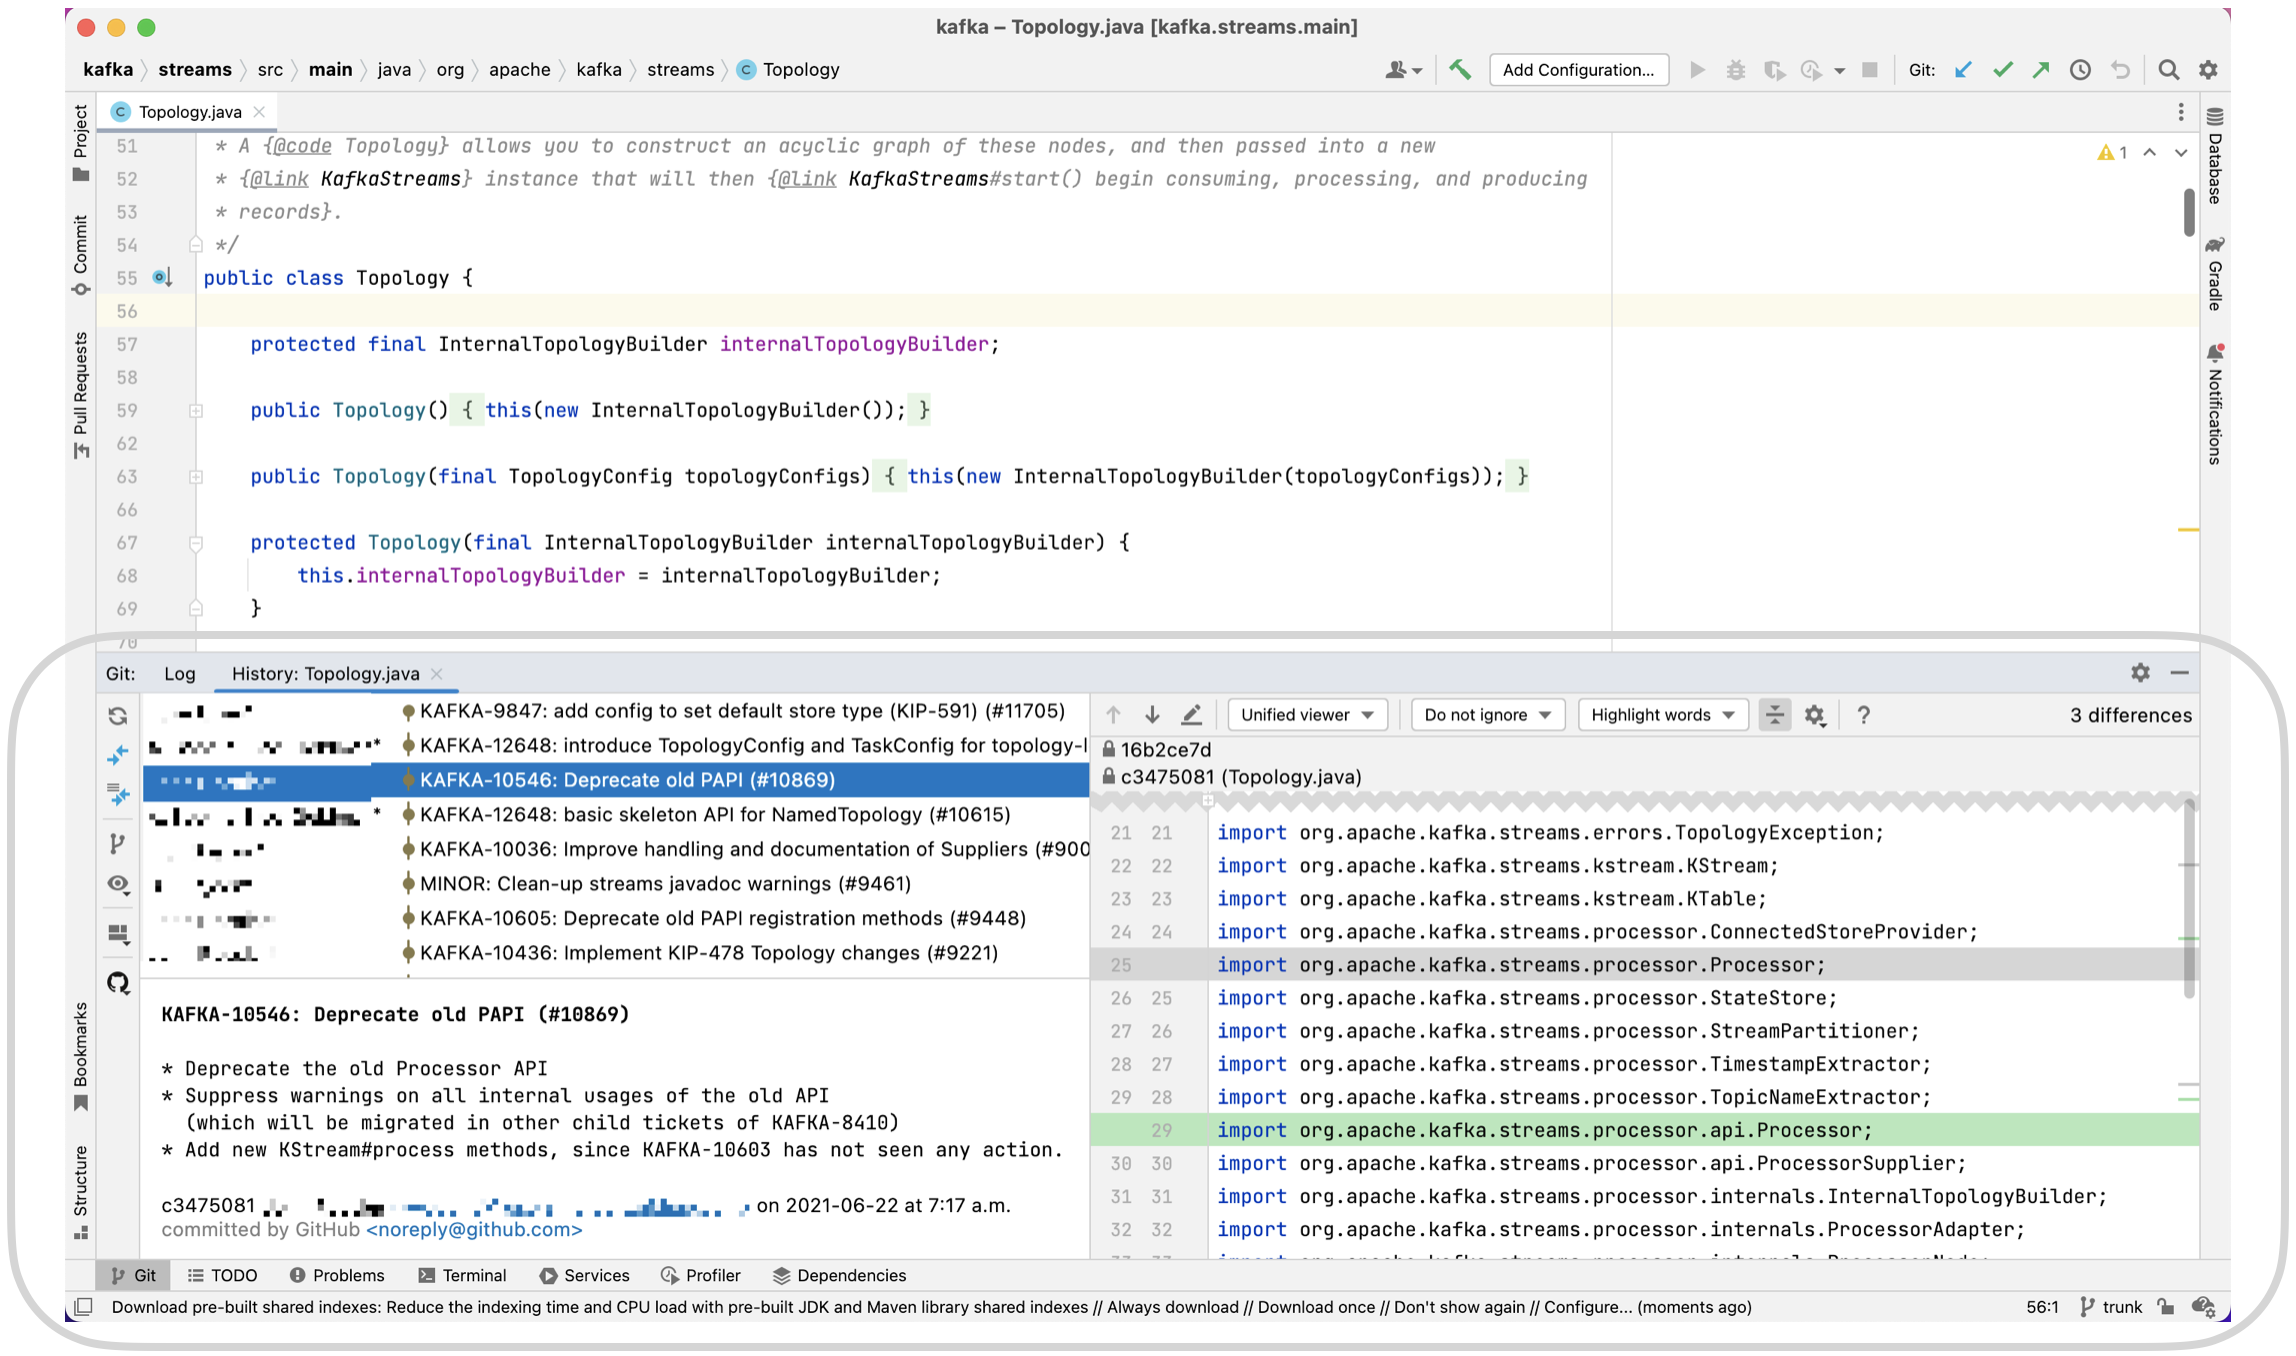
\includegraphics[width=\textwidth]{./images/intellij-overview.png}
    \caption{
        IntelliJ IDEA overview with the commit history for the currently open \class{Topology} class visible in the bottom half tool window.
    }
    \label{fig:IntelliJ-Overview}
\end{figure}

As a plugin, Intelligent History integrates with IntelliJ's ``Show History'' feature seamlessly as the plugin adds actions that can be invoked from a toolbar in IntelliJ's existing interface for exploring a file's commit history. 
This makes the features of Intelligent History complimentary to IntelliJ's existing version control interface.
We designed Intelligent History to support the following questions a developer might ask when searching for code rationale information in a file's revision history:

\begin{enumerate}[label={(\arabic*)}]
    \item \textit{Which commits are likely to be meaningful for understanding the decisions and choices involved in the evolution of this file?}
    \item \textit{Is there an interesting discussion or rationale that motivated the changes in a commit?}
\end{enumerate}

Intelligent History has the following features implemented as \emph{actions} in the IntelliJ Platform \entity{SDK}, which the user can invoke:

\begin{enumerate}[label=(\Alph*)]
    \item \textit{Highlight Important Changes}: A toggleable action that automatically detects less important commits and applies highlighting on a file's commit history to distinguish potentially important commits from less important commits. The determination of less important commits is based on a set of heuristics in the form regular expressions applied to the diff content of commits. The implementation of this heuristics-checking is described further in \autoref{sec:Heuristics}. \autoref{fig:Intelligent-History-A} demonstrates the highlighting action toggled on and applied to the commit history for a class.
    \item \textit{Show Diff Metadata}: An action that displays a pop-up summary of metadata information on the diff for a user-selected commit in a file's commit history. This summary contains a categorization of code changes in a commit's diff content and the number of lines detected in a diff according to the heuristics used for determining less important commits. The details on this categorization is also further explained in \autoref{sec:Heuristics}. \autoref{fig:Intelligent-History-B} shows an example of the metadata popup invoked for a selected commit.
    \item \textit{Show Jira Issue}: An action that extracts the Jira issue ID for a user-selected commit in a file's commit history and fetches and displays the Jira issue information in a dedicated tool window. The Jira issue ID is extracted from a commit's message using regular expressions. Along with the Jira issue information, this action also provides a meatdata summary of the Jira issue, which includes metrics on the number of comments on the Jira issue made by commit author, the total number of comments on the Jira issue exluding bot comments, the total number of unique people involved in the Jira issue based on comments including the Jira issue assignee, the number of people subscribed to the Jira issue (``watches''), the number of votes on the Jira issue, the number issue links, and the number of sub-tasks. \autoref{fig:Intelligent-History-C} illustrates the tool window showing the information extracted for an automatically identified Jira ID from a selected commit.
\end{enumerate}

These actions added by the Intelligent History plugin are indicated in \autoref{fig:Intelligent-History-Overview}, where the actions are presented as icons in IntelliJ's \entity{VCS} file history tool bar.

\begin{figure}[h]
    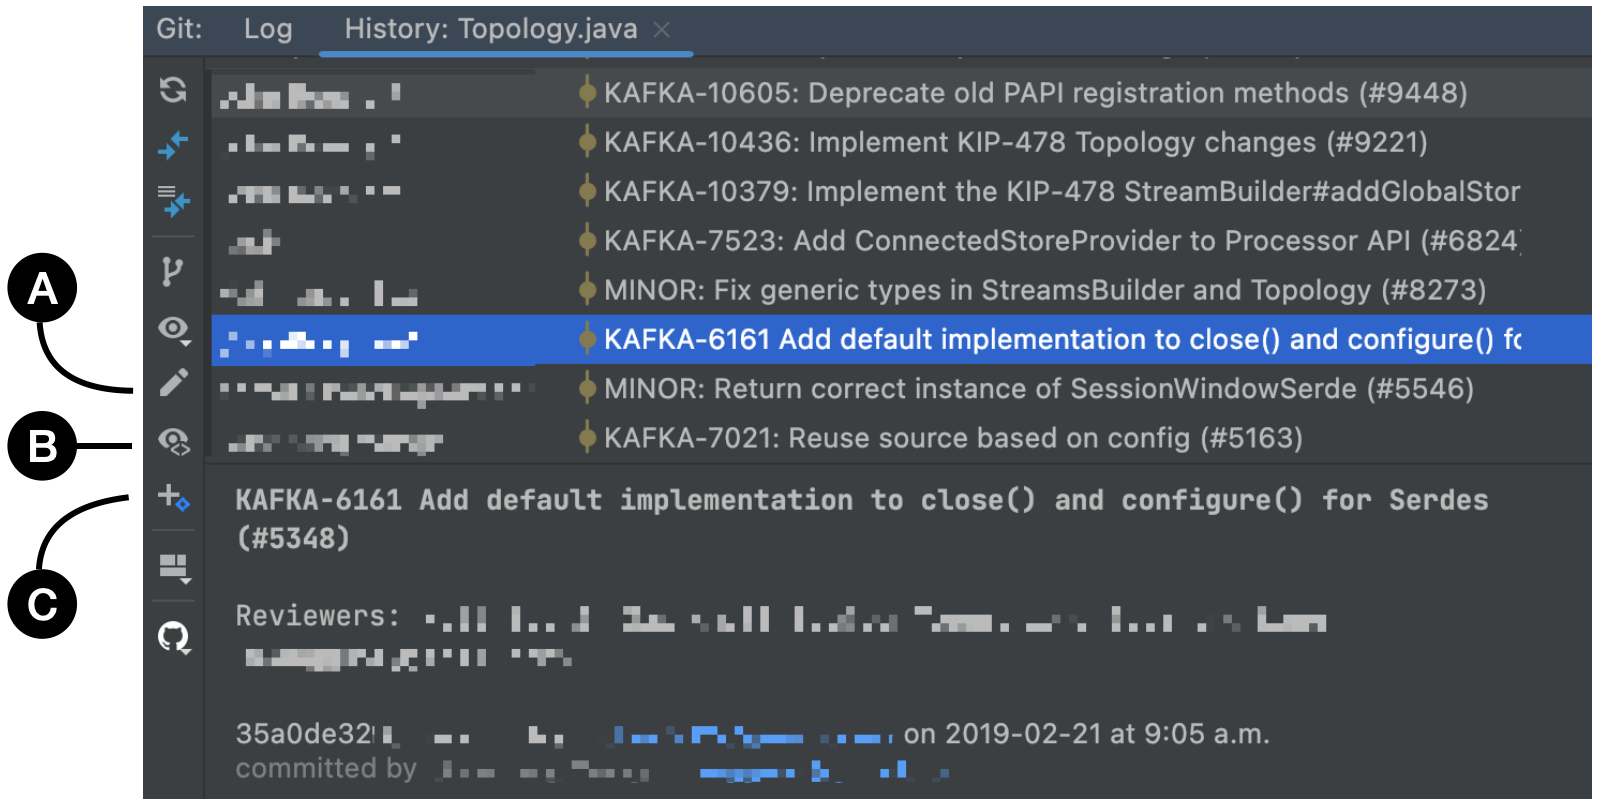
\includegraphics[width=\textwidth]{./images/intelligent-history-overview.png}
    \caption{
        Overview of the actions added by the Intelligent History plugin. We use the following labels: (A) \textit{Highlight Important Changes}; (B) \textit{Show Diff Metadata}; and (C) \textit{Show Jira Issue}.
    }
    \label{fig:Intelligent-History-Overview}
\end{figure}

\begin{figure}[h]
    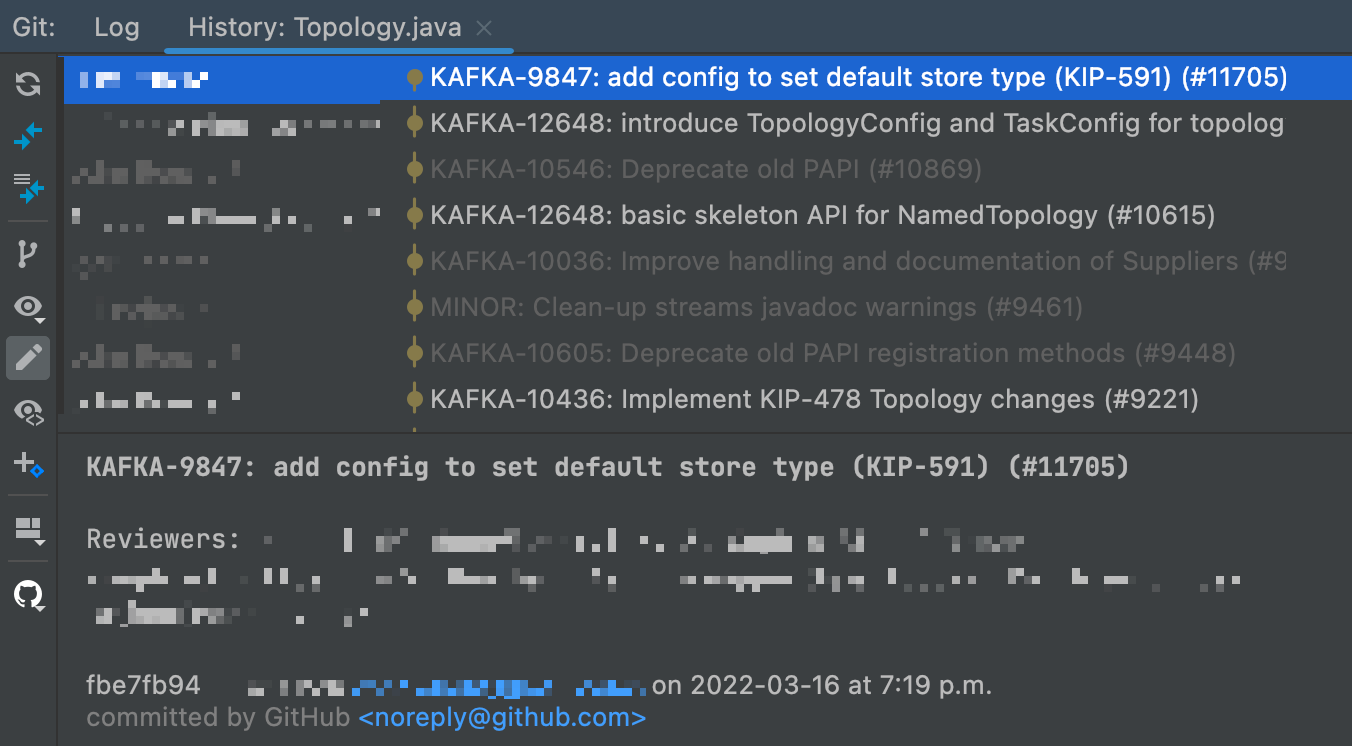
\includegraphics[width=\textwidth]{./images/intelligent-history-A.png}
    \caption{
        Feature (A) \textit{Highlight Important Changes} of Intelligent History in the toggled on state. Less important commits have been highlighted to blend with the foreground to make potentially more interesting commits stand out.
    }
    \label{fig:Intelligent-History-A}
\end{figure}

\begin{figure}[hp]
    \centering%
    \subfloat[\centering Popup \label{subfig:Intelligent-History-B-Popup}]{{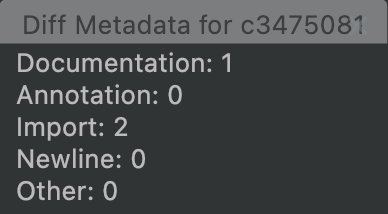
\includegraphics[width=4cm]{./images/intelligent-history-B-a.png}}}%
    \qquad
    \subfloat[\centering Diff \label{subfig:Intelligent-History-B-Diff}]{{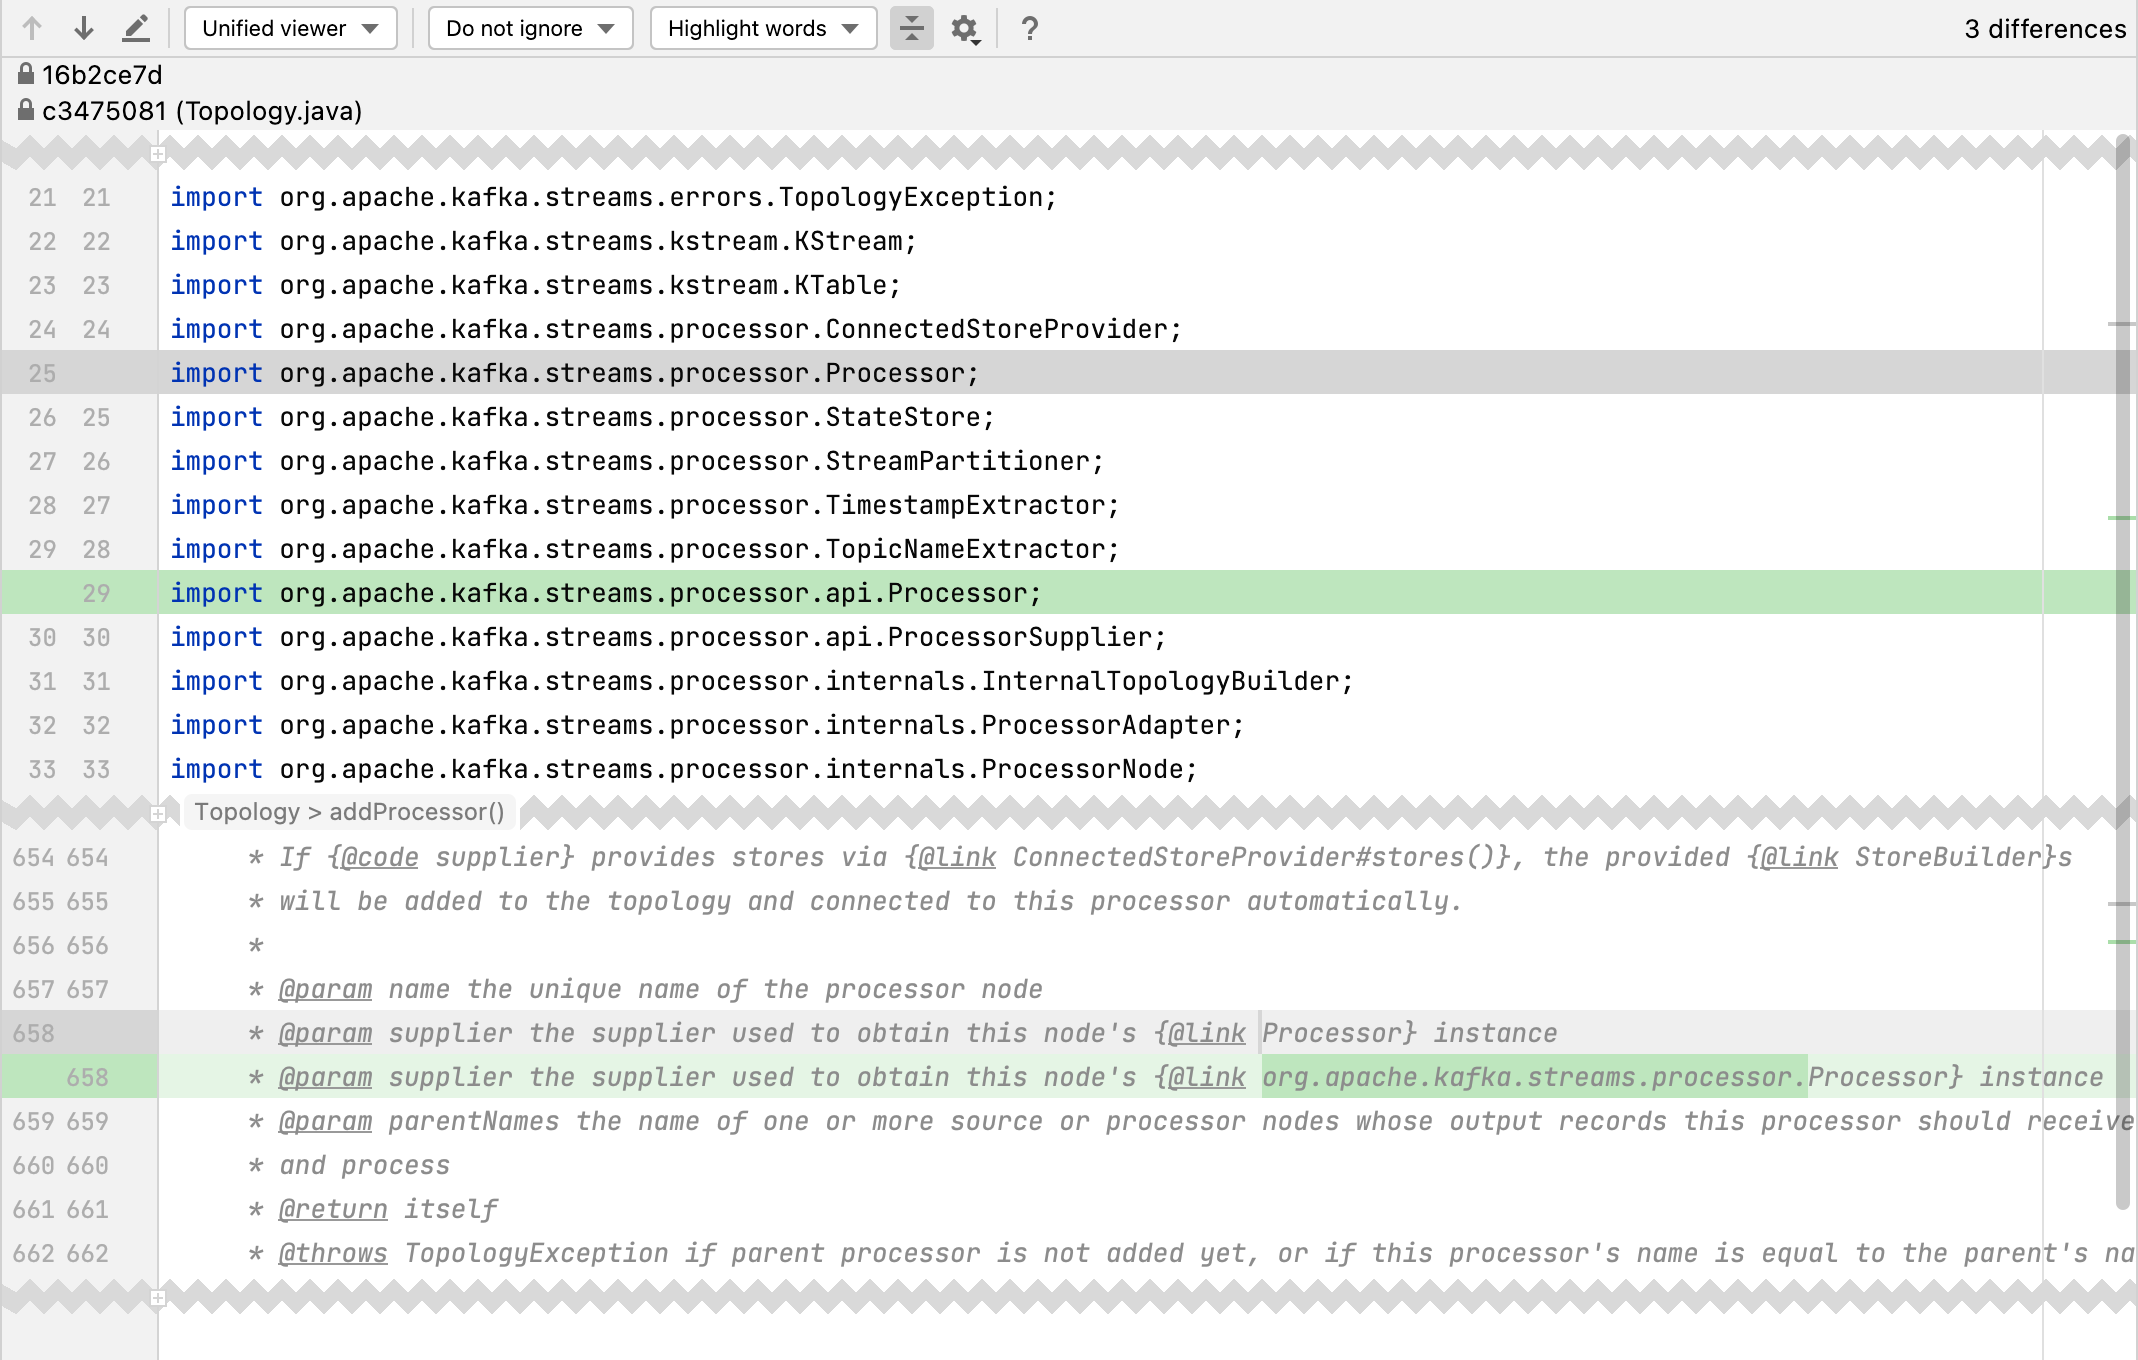
\includegraphics[width=10cm]{./images/intelligent-history-B-b.png}}}%
    \caption{
        Feature (B) \textit{Show Diff Metadata} invoked on commit \commit{c3475081}.\textsuperscript{*}
    }%
    \scriptsize\textsuperscript{*} \url{https://github.com/apache/kafka/commit/c3475081c5e8228e9bd3a45022a93d61e542f72e}
    \label{fig:Intelligent-History-B}%
\end{figure}

\begin{figure}[hp]
    \center
    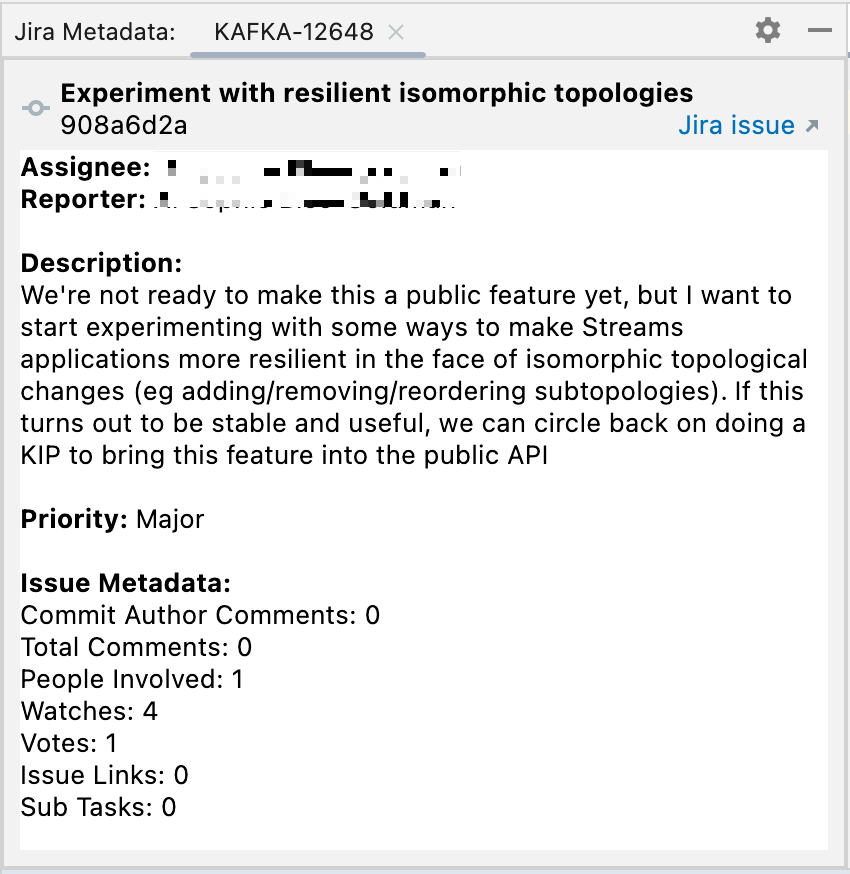
\includegraphics[width=7cm]{./images/intelligent-history-C.png}
    \caption{
        Feature (C) \textit{Show Jira Issue} invoked on commit \commit{908a6d2a}.\textsuperscript{*}
        Shows the explicitly referenced Jira issue's title, assignee, reporter, description, priority, and metadata in a tool window. A hyperlink to the Jira issue is also provided.
    }
    \scriptsize\textsuperscript{*} \url{https://github.com/apache/kafka/commit/908a6d2ad7807642b917231769c8d3b6a0c1ad16}
    \label{fig:Intelligent-History-C}
\end{figure}

%%%%%%%%%%%%%%%%%%%%%%%%%%%%%%%%%%%%%%%%%%%%%%%%%%%%%%%%%%%%%%%%%%%%%%
\section{Heuristics}
\label{sec:Heuristics}

For distinguishing potentially important commits from less important or trivial commits, we employ a heuristics-based approach to categorize the lines of change in a commit's diff content.
When referring to a commit's diff content, we mean the diff between the old version of a Java class in one commit, and the new version of the Java class after a commit has modified it.
This approach involves scanning the lines between commits for matches to a set of Java code patterns, which describe categories of trivial code changes.
Each pattern is expressed by a form of regular expressions.

While using regular expressions sacrifices some degree of accuracy on what is considered a ``trivial'' line of code change to a user,
regular expressions have the advantage of being lightweight in efficiency and interpretability over other approaches to detecting code changes in programs such as abstract syntax tree (\entity{AST}) matching and differencing techniques \cite{murphy_lightweight_1996}.
Though the advantage of \entity{AST}-level granularity is that it produces edit scripts that directly refer to the structure of code, \entity{AST} matching and differencing techniques having negative performance on runtime and memory consumption, which discouraged us from using them \cite{fluri_change_2007,pawlik_RTED_2011,falleri_fine-grained_2014}.
The goal of our approach is to understand if a minimal set of patterns for expressing trivial code changes can be effective at supporting a software developer in more efficiently navigating software history when searching for code rationale information.

Represented as regular expressions for the Java programming language, our approach for detecting trivial commits uses the following categories for a line of code that has been changed and expressed in a diff: 

\begin{itemize}
    \item \textit{Documentation}: Changes that insert, delete, or modify lines representing single-line or multi-line comments.
    \item \textit{Annotation}: Changes that modify lines representing \code{@Deprecated} annotations or annotations prefixed with \code{@Suppress}.
    \item \textit{Import}: Changes which involve the insertion, deletion, or modification of \code{import} statements.
    \item \textit{Newline}: Changes involving the insertion or deletion of newlines.
    \item \textit{Other}: Any change not classified by the above categories. If a commit has a diff containing at least one change that is not classified by any of the above categories, then the commit is regarded as potentially interesting. Else, a commit is considered less interesting and will be presented as a greyed out commit when the user invokes the \emph{Highlight Import Changes} action.
\end{itemize}

We use the \entity{java-diff-utils} \cite{java-diff-utils} library to extract the diff between two states of a file in the form of deltas. 
To obtain the state of a file for a given commit, we use the IntelliJ Platform's \entity{git4idea} library to retrieve the commits displayed in a file's commit history and the content of the file at the given commit.
The \entity{java-diff-utils} library provides a method that takes an old version $A$ and a new version $B$ of the contents of a file, represented as strings, and produces a list of \emph{abstract deltas} representing each change found from version $A$ to version $B$. 
Each delta contains a list of \emph{source lines} as strings and a list of \emph{target lines} as strings, where source lines represent consecutive lines in version $A$ and target lines represent consecutive lines in version $B$. 
For a set of consecutive lines that have changed from version $A$ to version $B$, a delta would contain the previous state of the lines in source lines and the new state of the lines in target lines.
For a delta that represents an insertion, the source lines would be empty, while the target lines would contain a list of the lines inserted in version $B$.
For a delta that represents a deletion, the target lines would be empty, while the source lines would contain a list of the lines deleted in version $B$.

For each commit in a file's commit history, beginning from the oldest commit to the most recent commit, we obtain the set of deltas for each sequential pair of commits.
Suppose we have a file $F$ and an ordered set of commits representing its commit history as $\{C_{1}, C_{2}, C_{3}, \dots, C_{n}\}$, where $C_{i}$ is a commit that affects $F$ and $i = 1, 2, 3, \dots, n$ denotes the oldest commit to the most recent commit in $F$'s commit history.
We use \entity{java-diff-utils} to obtain the diffs for the state of $F$ in the commit pairs $\{\varnothing, C_{1}\}$, $\{C_{1}, C_{2}\}$, $\{C_{2}, C_{3}\}$, \dots, $\{C_{n-1}, C_{n}\}$.
We compare an empty set, representing an empty string, with the state of $F$ in the first commit $C_{1}$ since the first commit in a file presumably introduces the file $F$ and its initial content.
For each pair of commits, we take the contents of file $F$ in each commit and  obtain a list of deltas and apply regular expression pattern matching on each string in a delta's list of source lines and list of target lines to count the number of lines that match a category.

This categorical information for a user-selected commit is exposed as \emph{diff metadata} in a pop-up when the user invokes the \textit{Show Diff Metadata} action provided by Intelligent History.
\autoref{subfig:Intelligent-History-B-Popup} illustrates the metadata information in a popup for the diff presented in Figure \autoref{subfig:Intelligent-History-B-Diff}.
As shown in \autoref{subfig:Intelligent-History-B-Diff}, the commit \commit{   16b2ce7d} for \class{Topology.java} consists of deleting an \code{import} statement, inserting an \code{import} statement, and the modification of a JavaDoc comment.
Exposing this metadata to the user allows the user to obtain a summary about the lines changed from one commit to another commit and to also understand how Intelligent History highlights commits in a file's commit history.

%%%%%%%%%%%%%%%%%%%%%%%%%%%%%%%%%%%%%%%%%%%%%%%%%%%%%%%%%%%%%%%%%%%%%%
\section{Predictions}
\label{sec:Predictions}

With the features of Intelligent History established in \autoref{sec:Implementation}, we describe how we anticipate a user might be able to use the actions from Intelligent History. 
In \autoref{sec:Implementation}, we outlined the three actions a user can invoke while examining a file's history using IntelliJ's built-in file revision history view: (A) \textit{Highlight Important Changes}; (B) \textit{Show Diff Metadata}; and (C) \textit{Show Jira Issue}.

%%%%%%%%%%%%%%%%%%%%%%%%%%%%%%%%%%%%%%%%%%%%%%%%%%%%%%%%%%%%%%%%%%%%%%
\endinput

Any text after an \endinput is ignored.
You could put scraps here or things in progress.